\subsection{Enunciado}
\begin{frame}
	\begin{block}{viajante de comercio con vuelta atrás y ramificación y poda.}
	Cuando para un nivel no queden más ciudades válidas, el algoritmo hace una vuelta atrás 
	proponiendo una nueva ciudad válida para el nivel anterior.

	Para el algoritmo de ramificación y poda es necesario utilizar una cota inferior para cada nodo 
	(solución parcial), un valor $c$ menor o igual que el verdadero coste de la mejor solución (la de 
	menor coste) que se puede obtener a partir de la solución parcial en la que nos encontremos.

	Para realizar la poda, guardamos en todo momento en una variable $C$ el costo de la mejor solución
	obtenida hasta ahora, si para una solución parcial, $c>C$ entonces se puede podar.

	Como criterio para seleccionar el siguiente nodo vivo se empleará el criterio LC o 
	``más prometedor", aquel que presente el menor valor de cota inferior.
	\end{block}
\end{frame}


\subsection{Explicación}
\begin{frame}

\end{frame}


\subsection{Eficiencia}
\begin{frame}

\end{frame}


\subsection{Comparativa}
\begin{frame}{Comparativa}
	\begin{block}{Funciones de cota}
	Las diferentes funciones para conseguir una cota inferior hacen que en un mismo mapa
	el algoritmo de ramificación y poda varíe. 
	\end{block}
	
	\begin{exampleblock}{Datos}
	\begin{itemize}
		\item Nodos expandidos
		\item Mayor cola de nodos vivos
		\item Cantidad de cortes
		\item Tiempo
	\end{itemize}
	\end{exampleblock}
\end{frame}



\subsubsection{Cortes producidos}
\begin{frame}{Cortes}
	\begin{block}{Representatividad}
	Esta información puede no ser representativa de la
	magnitud de los cortes. Dados dos algoritmos $X,Y$ que han hecho $x_i,y_i$ cortes
	respectivamente con $x_1>y_1$ no nos está diciendo que el primero sea más rapido.
	El primer algoritmo podría haber recorrido más nodos y hacer los cortes en niveles 
	del árbol más profundos. 
	\end{block}
\end{frame}
 
\begin{frame}
	\begin{exampleblock}{Imagen}
	\begin{figure}[H]
    		\centering
	%    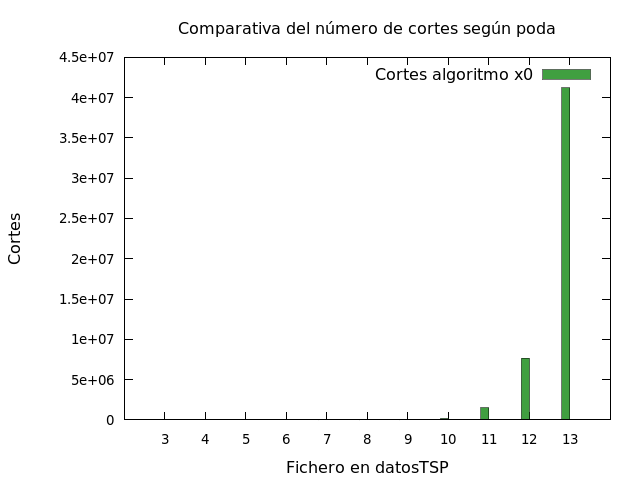
\includegraphics[scale=0.75]{../TSP/Graficas/graficaCortes.png}
    		\caption{Cortes efectuados}
	\end{figure}
	\end{exampleblock}
\end{frame}


\subsubsection{Colas con prioridad}
\begin{frame}{Tamaño de la lista de nodos vivos}
	\begin{block}{ }
	A continuación exponemos el mayor tamaño alcanzado por la cola con prioridad.
	Esta información nos puede dar una idea de lo bueno que es nuestro algoritmo 
	para el cálculo de una cota inferior.
	\end{block}
	
	\begin{block}{Otras versiones}
	Hay versiones de ramificación y poda para el problema del viajante
	de comercio que no usan por ejemplo la aproximación greedy inicial, por lo que ha podido 
	sobrecargar la cola con prioridad mientras busca la primera solución con la que podará después.
	\end{block}
\end{frame}

\begin{frame}
	\begin{exampleblock}{Imagen}
	\begin{figure}[H]
    		\centering
	%    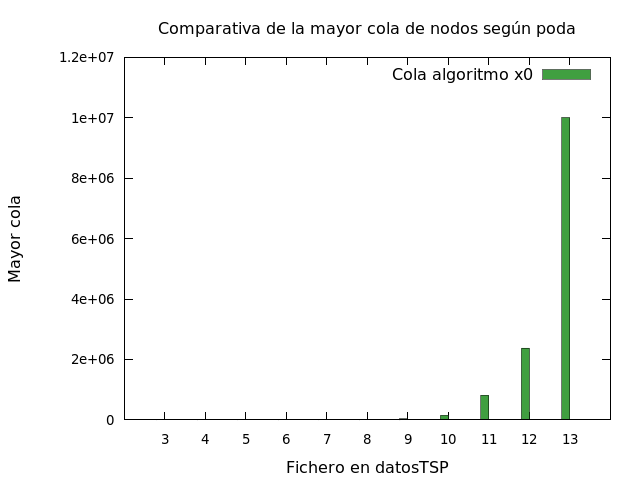
\includegraphics[scale=0.75]{../TSP/graficaColaMaxima.png}
    		\caption{Cola con prioridad más grande}
	\end{figure}
	\end{exampleblock}
\end{frame}


\subsubsection{Nodos procesados}
\begin{frame}{Nodos}
	\begin{block}{Utilidad}
	Este dato no nos asegura que tarde menos tiempo, ya que un algoritmo con más nodos 
	expandidos que otro ha podido usar una función para calcular las cotas inferiores demasiado costosa.
	\end{block}
\end{frame}

\begin{frame}
	\begin{exampleblock}{Imagen}
	\begin{figure}[H]
    		\centering
	%    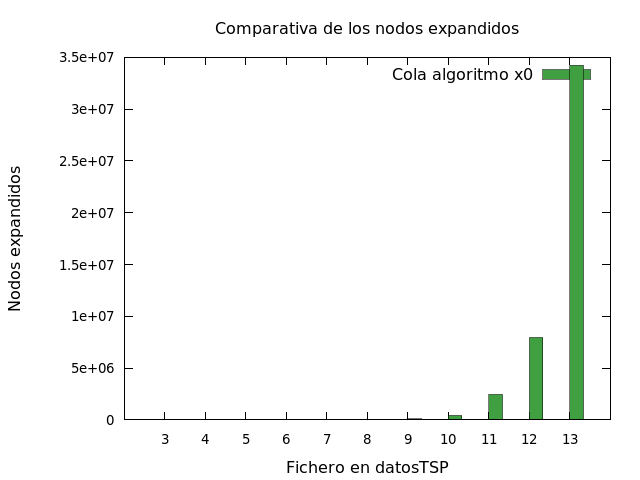
\includegraphics[scale=0.75]{../TSP/graficaNodos.png}
    		\caption{Nodos expandidos}
	\end{figure}
	\end{exampleblock}
\end{frame}


\subsubsection{Tiempos}
\begin{frame}
	\begin{exampleblock}{Imagen}
	\begin{figure}[H]
    		\centering
	%    \includegraphics[scale=0.75]{../TSP/graficaTiempos0.png}
    		\caption{Tiempo algoritmo 1 y su ajuste}
	\end{figure}
	\end{exampleblock}
\end{frame}

\begin{frame}
	\begin{exampleblock}{Imagen}
	\begin{figure}[H]
    		\centering
	%    \includegraphics[scale=0.75]{../TSP/graficaTiempos1.png}
    		\caption{Tiempo algoritmo 2 y su ajuste}
	\end{figure}
	\end{exampleblock}
\end{frame}


\begin{frame}
	\begin{exampleblock}{Imagen}
	\begin{figure}[H]
    		\centering
	%    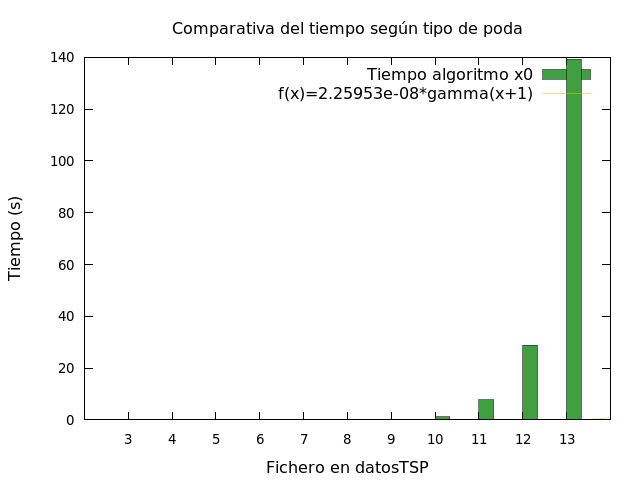
\includegraphics[scale=0.75]{../TSP/graficaTiempos.png}
    		\caption{Comparativa de tiempos}
	\end{figure}
	\end{exampleblock}
\end{frame}



\subsection{Conclusión}
\begin{frame}
	\begin{alertblock}
	Aunque los algoritmos de ramificación y poda nos aseguraran la optimalidad a problemas con
	tiempos de ejecución exponenciales ahorrándonos pasos, no resultan prácticos cuando el tamaño
	del problema crece. Los algoritmos greedy estudiados anteriormente nos pueden dar una 
	aproximación más que razonable para el problema.
	\end{alertblock}
\end{frame}
